\chapter{Komunikační modul Wireless M-Bus}

Spolu se zařízením UniPi Neuron S103 byl zapůjčen i modul IQRF TR-72DC-WMB, který do budoucna bude součástí tohoto produktu a bude rozšiřovat konektivitu zařízení o protokol Wireless M-Bus. 

\section{Obecný popis modulu TR-72D-WMB}

Modul IQRF TR-72DA-WMB je bezdrátový komunikační modul velikosti SIM karty z výroby české firmy \href{http://microrisc.com/cs/}{MICRORISC s.r.o.}. Vychází z řady produktů technologie IQRF, s tím rozdílem, že místo IQRF softwaru má přímo implementovaný Wireless M-Bus protokol \cite{iqrfmodul}. 

 \begin{figure}[!h]
  \begin{center}
    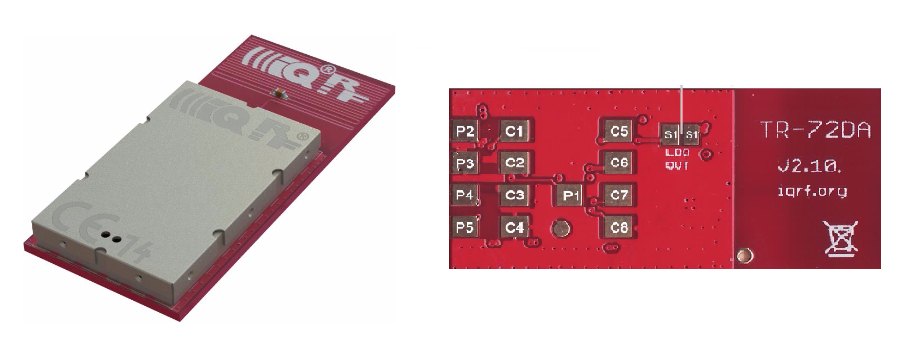
\includegraphics[scale=0.6]{obrazky/modul_modul}
  \end{center}
  \caption{Modul IQRF TR-72DA-WMB \cite{iqrfmodul}}
\end{figure}

Na malém prostoru se nachází vše potřebné pro uskutečnění bezdrátového přenosu: mikrokontrolér, externí EEPROM, teplotní senzor, kontrolní LED , 6 pinů a anténa dle typu komunikačního modulu (Obr.\label{BlokovkaIQRF}).



Modul podporuje módy přenosu S1, S2, T1 a T2. Napájecí napětí modulu je v rozsahu 3.1 až 5.3\,V se spotřebou 1\,$\mu$A v režimu spánku a 8-22\,mA ve vysílacím režimu, dle nastavení výstupního výkonu, jehož maximální hodnota je 12.5\,W.
V České republice je využíván pro přenos v bezlicenčním pásmu 868\,MHz, případně 433\,MHz a je možno jej přizpůsobit na vysílání v pásmu 916\,MHz, určené pro okolní státy.\newline

\newpage

 \begin{figure}[!h]
  \begin{center}
    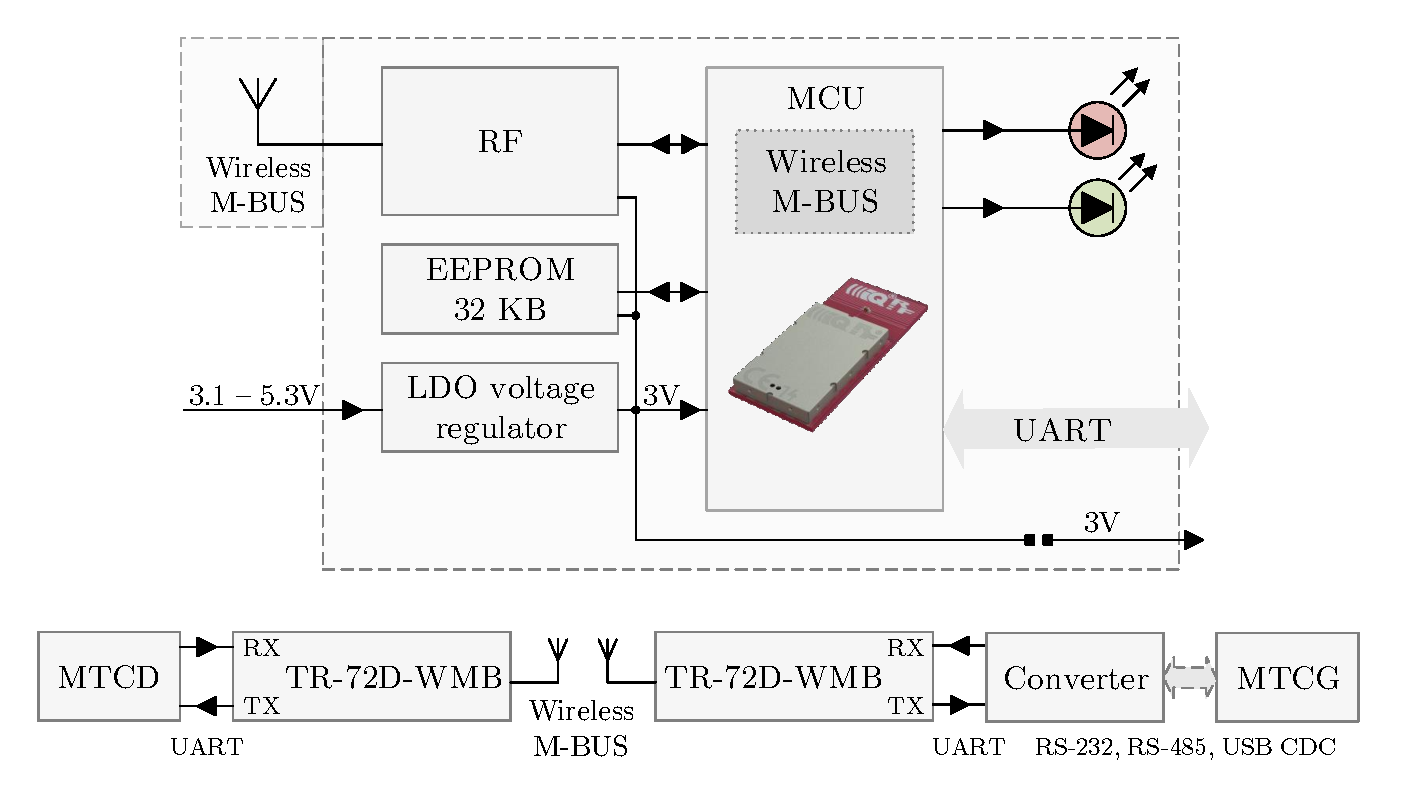
\includegraphics[scale=0.6]{obrazky/modul_block}
  \end{center}
  \caption{Blokové schéma modulu TR-72D-WMB \cite{iqrfmodul}}
	\label{BlokovkaIQRF}
\end{figure}

Modul lze pořídit ve třech verzích (Obr.\label{ObrazekAnteny}) dle připojení antény:
\begin{itemize}
		\item TR-72D-WMB má zdířku pro připájení antény.
		\item TR-72DC-WMB	má vyveden koaxiální anténí konektor U.FL. 
		\item TR-72DA-WMB má integrovanou anténu přímo na desce modulu. Dosah signálu toto typu je až 320\,m v módu T a 365\,m v módu S.
\end{itemize}
 \begin{figure}[!h]
  \begin{center}
    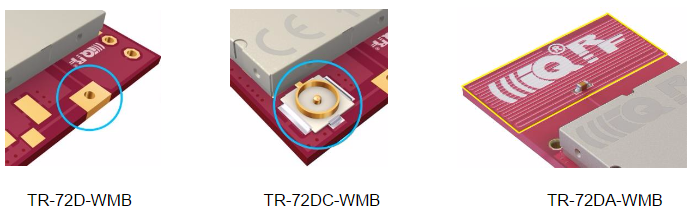
\includegraphics[scale=0.7]{obrazky/modul_antena}
  \end{center}
  \caption{Prehled typu modulu dle anteny \cite{iqrfmodul}}
	\label{ObrazekAnteny}
\end{figure}

\section{Komunikační módy}

Modul může být v závislosti na použité topologii nastaven do jednoho ze tří provozních módů: měřič, koncentrátor, skener \cite{iqrfmodul}. 

V módu měřiče může být modul přes UART sběrnici zapojen k mikrokontroléru, který zajistí zpracování dat od senzorů. Může tedy sloužit k sestavení vlastních měřicích zařízení postavených na protokolu Wireless M-Bus.

V módu koncentrátoru slouží modul jako komunikační zařízení pro sběr dat z meřičů. Aktuální firmware podporuje pouze obousměrnou komunikaci s měřiči v režimu S a T a je zatím ve fázi vývoje a do produkce nasazena jako experimentální. Z tohoto důvodu bude při implementaci samotné aplikace modul nasazen v režimu skeneru.

V módu skeneru modul zachytává veškerou dostupnou komunikaci daného módu přenosu. Díky vnitřní implementaci Wireless M-Bus protokolu je modul schopen zachytávat a dešifrovat šifrovanou komunikaci, je vsak nutne pocitat s tim, ze soucasny firmware neni staveny na vyuziti v modu skeneru pro prijem sifrovane komunikace. Modul totiz automaticky veskere zachycene sifrovane telegramy automaticky rozsifruje pomoci jedineho interniho AES klice. Jedna se vsak o klic daneho modulu, nikoliv vycitaneho zarizeni. Pri vycitani sifrovanych dat je tedy nutne postupovat sloziteji a provest nejdrive zpetne zasifrovani danych dat timto klicem a pote az provest rozsifrovani dle normy, blize popsane v sekci \ref{section_unencrypted_communication}.

Praktické využíti jednotlivých módu zobrazuje obrázek \ref{TopologieIQRF}.

 \begin{figure}[!h]
  \begin{center}
    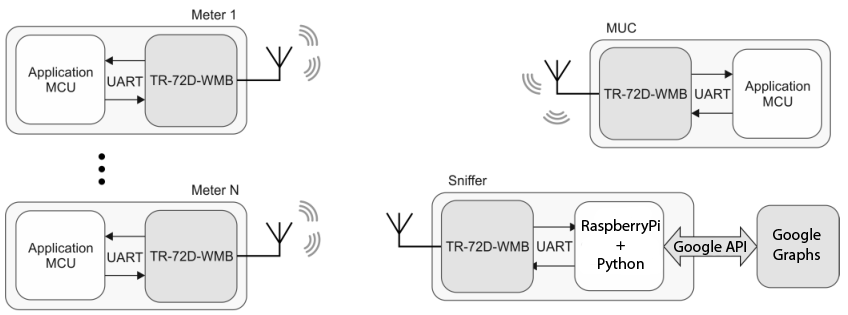
\includegraphics[scale=0.6]{obrazky/modul_topologie}
  \end{center}
  \caption{Různé módy dle použité topologie \cite{iqrfmodul}}
	\label{TopologieIQRF}
\end{figure}

\section{Komunikační protokol}

S řídícím mikrokontrolérem modul komunikuje pomocí rozhraní UART, jehož parametry jsou 19200\,Bd, 8\,bitů, žádná parita a 1 stop bit.
		
 \begin{figure}[!h]
  \begin{center}
    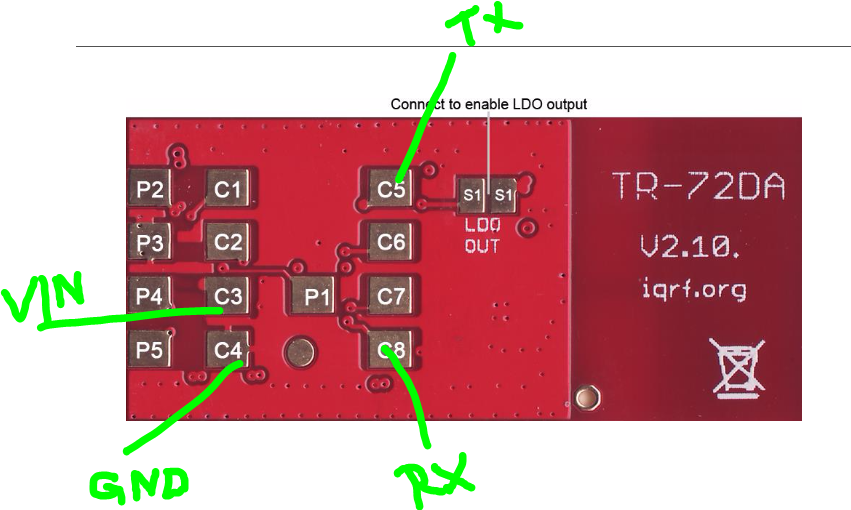
\includegraphics[scale=0.4]{obrazky/modul_zada}
  \end{center}
  \caption{Zadní strana modulu s popisem pinů \colorbox[rgb]{0,1,0}{bude překreslen}}
\end{figure}

Modul podporuje jednoduchý formát příkazů sloužící k nastavení konfiguračních parametrů modulu i ke samotné komunikaci s modulem. Každý příkaz začíná znakem \textbf{\textgreater}. Každá zpráva odpověďi začíná znakem \textbf{\textless}. Každému příkazu musí předcházet budící znak NULL (\textbf{0x00}) následovaný 2\,ms pauzou a každý paket příkazů je ukončen znakem CR (\textbf{0x0D}). 

Obecná struktura\cite{iqrfmodul} paketu příkazu je 

\begin{eqnarray}
	>[CC][RW][DATA][CR]
\end{eqnarray}

kde CC je jednobajtový kód daného příkazu, RW je jednobajtový příznak zápisu (\textbf{:}) či čtení dat (\textbf{?}) dat, DATA jsou zapisovaná data, pokud se jedná o zápis a CR je znak ukončení.

Obecná skruktura odpovědi je následující

\begin{eqnarray}
	<[DATA][CR]
\end{eqnarray}

kde DATA obsahuje přenášená data či návratové kódy (OK pro správné dokončení příkazu, ERR1 pro chybu syntaxe a ERR2 pro neplatnou vstupní hodnotu). Některé bajty jsou kódovány v šestnáckové soustavě či využívají uložení BigEndian.

Například dotaz a odpověd pro aktuální AES klíč je:

\begin{eqnarray}
	>03?[CR]
	<010203040506070809a0b0c0d0e0f[CR]
\end{eqnarray}

a pro případnou změnu AES klíče:

\begin{eqnarray}
>03:112233445566778899aabbccddeeff[CR]\\
>OK[CR]
\end{eqnarray}

Pri prenosu datove jednotky uvedene v Tab. \ref{PaketWm3} modulem dochazi k jejimu rozsireni o polozky uvedene v Tab. \ref{PaketWm4}.

\begin{table}[!h]
\centering
\begin{tabular}{ccccccc}
1 Bajt & 1 Bajt & 12\,-\,n Bajtu & 1 Bajt & 1 Bajt & 1 Bajt & 1 Bajt\\ \hline
\multicolumn{1}{|c|}{Length} & \multicolumn{1}{c|}{Status} & \multicolumn{1}{c|}{...} & \multicolumn{1}{c|}{CRC} & \multicolumn{1}{c|}{RSSI} & \multicolumn{1}{c|}{CR} & \multicolumn{1}{c|}{0A}\\ \hline
\end{tabular}
\caption{Format datove jednotky po prijeti modulem IQRF}
\label{PaketWm4}
\end{table}

Bližší popis jednotlivých podporovaných příkazů je součástí \hyperlink{prilohaB}{přílohy B} této práce.





